\documentclass[11pt,a4paper,fontset=fandol]{ctexart}

\usepackage[margin=1.78cm,top=1.85cm,bottom=1.9cm]{geometry}
\usepackage{booktabs}
\usepackage{longtable}
\usepackage{array}
\usepackage[table]{xcolor}
\usepackage{hyperref}
\usepackage{fancyhdr}
\usepackage{lastpage}
\usepackage{titlesec}
\usepackage{needspace}
\usepackage{tabularx}
\usepackage{tikz}
\usepackage{enumitem}
\usepackage{xurl}

\hypersetup{colorlinks=true,linkcolor=navy,urlcolor=teal}
\setlength{\parindent}{2em}
\setlength{\parskip}{0.32em}
\setlength{\headheight}{15pt}
\setlength{\emergencystretch}{3em}
\renewcommand{\arraystretch}{1.18}
\sloppy

\definecolor{navy}{HTML}{17324D}
\definecolor{teal}{HTML}{117A79}
\definecolor{green}{HTML}{18794E}
\definecolor{red}{HTML}{A13A3A}
\definecolor{amber}{HTML}{B66A12}
\definecolor{muted}{HTML}{6B7280}
\definecolor{lightblue}{HTML}{EEF4F8}
\definecolor{lightteal}{HTML}{E9F6F4}
\definecolor{lightamber}{HTML}{FFF5E7}
\definecolor{lightgray}{HTML}{F3F4F6}
\definecolor{linegray}{HTML}{D7DEE5}

\newcommand{\Pass}{\textcolor{green}{\textbf{通过}}}
\newcommand{\Fail}{\textcolor{red}{未通过}}
\newcommand{\Untested}{\textcolor{muted}{未评测}}
\newcommand{\Tpass}{\textcolor{green}{\textbf{通过}}}
\newcommand{\Tfail}{\textcolor{red}{未过}}
\newcommand{\Tuntested}{\textcolor{muted}{未测}}
\newcommand{\code}[1]{\texttt{\detokenize{#1}}}
\newcommand{\metric}[3]{%
  \begin{minipage}[c][2.15cm][c]{0.285\textwidth}
  \centering
  \textcolor{#3}{\fontsize{24}{27}\selectfont\textbf{#1}}\\[-0.05em]
  \small #2
  \end{minipage}}

\titleformat{\section}{\Large\bfseries\color{navy}}{\thesection}{0.65em}{}
\titleformat{\subsection}{\large\bfseries\color{navy}}{\thesubsection}{0.65em}{}

\pagestyle{fancy}
\fancyhf{}
\lhead{GLM-5.2 三系统总对比}
\rhead{2026-07-22}
\cfoot{第 \thepage\ 页}

\begin{document}

\begin{titlepage}
\pagecolor{lightblue}
\color{navy}
\vspace*{2.2cm}
\begin{center}
{\fontsize{29}{35}\selectfont\bfseries GLM-5.2 在三种 Agent 系统上的\\[0.22em]SWE-bench Pro-Lite 总对比报告}

\vspace{0.8cm}
{\Large OpenHands、Claude Code 与 OpenCollab G1.1}

\vspace{1.3cm}
\begin{tikzpicture}
\fill[teal] (0,0) rectangle (12.8,0.08);
\end{tikzpicture}

\vspace{1.2cm}
\colorbox{white}{\begin{minipage}{0.91\textwidth}
\centering
\metric{19/100}{OpenCollab G1.1}{navy}
\metric{16/100}{OpenHands}{teal}
\metric{15/100}{Claude Code}{amber}
\end{minipage}}

\vfill
{\large 署名\quad 拱垲}\\[0.4em]
{\large 2026 年 7 月 22 日}
\end{center}
\end{titlepage}
\nopagecolor

\begin{abstract}
本报告统一比较 GLM-5.2 在 OpenHands、Claude Code 与 OpenCollab G1.1 三种 Agent 系统上的 SWE-bench Pro-Lite 结果。OpenCollab G1.1 完整评测 100 题并通过 19 题，OpenHands 完整评测 100 题并通过 16 题，Claude Code 完整评测 100 题并通过 15 题。三者共同通过 11 题，三者通过并集为 23 题。报告给出完整百题对比、交并差集合、关键失败机制和 100 题逐题矩阵。
\end{abstract}

\tableofcontents
\newpage

\section{最终结果}

OpenCollab G1.1 的通过题号为 7、11、21、32、34、35、36、37、43、46、47、50、53、60、69、74、75、92、93。OpenHands 的通过题号为 7、11、21、32、33、34、53、55、60、69、70、74、75、78、92、93。Claude Code 的通过题号为 7、11、21、32、33、34、37、53、55、60、69、70、74、92、93。

三者共同通过 11 题，题号为 7、11、21、32、34、53、60、69、74、92、93。三者通过题目的并集为 23 题。三套系统均已完成 100 题最终能力分类，技术失败为 0。

\begin{center}
\rowcolors{2}{lightgray}{white}
\begin{tabular}{lrrrrr}
\toprule
系统 & 已评测 & 通过 & 未通过 & 技术失败 & 未评测 \\
\midrule
OpenCollab G1.1 & 100 & 19 & 81 & 0 & 0 \\
OpenHands & 100 & 16 & 84 & 0 & 0 \\
Claude Code & 100 & 15 & 85 & 0 & 0 \\
\bottomrule
\end{tabular}
\end{center}

\subsection{完整百题对比}

三套系统都完成了相同 100 题。OpenCollab G1.1 通过 19 题，比例为 19\%。OpenHands 通过 16 题，比例为 16\%。Claude Code 通过 15 题，比例为 15\%。

\begin{center}
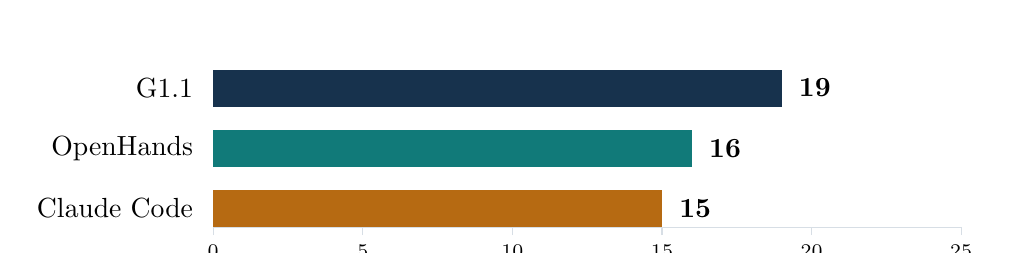
\begin{tikzpicture}[x=0.38cm,y=0.85cm]
\draw[linegray] (0,0.3) -- (25,0.3);
\fill[navy] (0,2.1) rectangle (19,2.65);
\fill[teal] (0,1.2) rectangle (16,1.75);
\fill[amber] (0,0.3) rectangle (15,0.85);
\node[anchor=east] at (-0.35,2.38) {G1.1};
\node[anchor=east] at (-0.35,1.48) {OpenHands};
\node[anchor=east] at (-0.35,0.58) {Claude Code};
\node[anchor=west,font=\bfseries] at (19.25,2.38) {19};
\node[anchor=west,font=\bfseries] at (16.25,1.48) {16};
\node[anchor=west,font=\bfseries] at (15.25,0.58) {15};
\foreach \x in {0,5,10,15,20,25} {\draw[linegray] (\x,0.18)--(\x,0.3); \node[below,font=\scriptsize] at (\x,0.18) {\x};}
\end{tikzpicture}
\end{center}

三套结果使用相同的百题分母，最终覆盖可以直接比较。G1.1 比 OpenHands 多通过 3 题，比 Claude Code 多通过 4 题。OpenHands 比 Claude Code 多通过 1 题。三方通过并集仍为 23 题，后续章节用这个重点切片分析各系统的重合与差异。

\section{交集、差集与覆盖结构}

\begin{center}
\begin{tabularx}{0.98\textwidth}{>{\raggedright\arraybackslash}p{4.2cm}>{\centering\arraybackslash}p{1.4cm}X}
\toprule
通过组合 & 题数 & 题号 \\
\midrule
三者共同通过 & 11 & 7、11、21、32、34、53、60、69、74、92、93 \\
G1.1 与 OpenHands 通过 & 1 & 75 \\
G1.1 与 Claude Code 通过 & 1 & 37 \\
OpenHands 与 Claude Code 通过 & 3 & 33、55、70 \\
仅 G1.1 通过 & 6 & 35、36、43、46、47、50 \\
仅 OpenHands 通过 & 1 & 78 \\
仅 Claude Code 通过 & 0 & 无 \\
\bottomrule
\end{tabularx}
\end{center}

G1.1 与 OpenHands 共同通过 12 题。G1.1 与 Claude Code 共同通过 12 题。OpenHands 与 Claude Code 共同通过 14 题。按 Jaccard 相似度计算，三组数值依次为 52.2\%、54.5\% 和 82.4\%。OpenHands 与 Claude Code 的通过集合最接近，14 道共同题覆盖 OpenHands 通过集合中的 87.5\%。

三者通过题目的并集为 23 题，其余 77 题由三套系统共同归为未通过。Claude Code 没有形成三者之外的独有通过题。23 题重点切片反映已有通过题的复现与互补结构，完整成绩统一采用百题分母。

\section{分段表现}

\begin{center}
\begin{tabular}{lccc}
\toprule
题号范围 & G1.1 通过 & OpenHands 通过 & Claude Code 通过 \\
\midrule
1--25 & 3/25 & 3/25 & 3/25 \\
26--50 & 9/25 & 3/25 & 4/25 \\
51--75 & 5/25 & 7/25 & 6/25 \\
76--100 & 2/25 & 3/25 & 2/25 \\
\bottomrule
\end{tabular}
\end{center}

G1.1 的独有优势集中在 26--50 区间。该区间包含 35、36、43、46、47、50 六道仅 G1.1 通过的题，也包含 37 这一道 G1.1 与 Claude Code 共同通过的题。OpenHands 与 Claude Code 的共同优势分布更分散，33 位于第二段，55 与 70 位于第三段。

\needspace{10\baselineskip}
\section{系统差异分析}

\subsection{OpenCollab G1.1 的跨模块覆盖}

仅 G1.1 通过的 35、36、43、46、47、50 涉及模块位置、公开接口、错误分类、端点会话结构、边界处理和回归兼容。Claude Code 在第 35 题把实现放进错误模块，在第 43 题只留下测试改动，在第 46 与 47 题遗漏接口结构，在第 50 题引入保留测试回归。G1.1 这一完整系统组合在这组跨模块任务上呈现更高的最终覆盖。

第 37 题由 G1.1 与 Claude Code 共同通过，OpenHands 未通过。这个结果显示 G1.1 的独有集合之外仍存在与 Claude Code 重合的跨模块任务，差异主要出现在更复杂的模块边界和兼容性题目上。

\subsection{OpenHands 与 Claude Code 的高度重合}

OpenHands 的 16 道通过题中有 14 道也被 Claude Code 做出。双方共同而 G1.1 未通过的 33、55、70 分别来自 OpenLibrary、ProtonMail WebClients 与 Navidrome。Claude Code 在 OpenHands 独有四题中复现三题，两种完整系统组合在这批题上的通过集合高度重合。

第 78 题只有 OpenHands 通过。Claude Code 修改了 OpenLibrary 的模型模块，公开目标要求的函数位于 catalog 工具模块，最终在导入阶段终止。该题体现了代码实现本身接近目标时，公开接口定位仍会决定最终结果。

\subsection{双方共同题上的稳定性}

G1.1 与 OpenHands 共同通过 12 题，Claude Code 复现其中 11 题。第 75 题成为唯一例外。Claude Code 的 TestCore 实际执行 44 项，其中 43 项通过，1 项失败。候选完成主要功能，同时引入一个可观测回归，因此最终归为未通过。

三者共同通过的 11 题跨越 Vuls、OpenLibrary、qutebrowser、NodeBB、Flipt 等项目。这 11 题在三种完整系统组合下都得到通过终态，呈现出跨系统的一致覆盖。

\section{关键题号与证据解释}

第 35 与 78 题均生成可信非空候选，追加 official eval 仍在公开目标导入阶段终止。第 35 题的实现位于错误模块，第 78 题缺少目标导入的公开函数。底层执行记录保留零目标事实，最终能力分类归为未通过。

第 43 题生成 2883 字节原始补丁，改动全部属于测试文件。候选发布时剔除模型写入的测试，评测补丁变为空。这个结果说明模型没有提供可接受的生产代码修复，最终能力分类同样归为未通过。

第 50 题的新行为目标通过，文件夹扩展属性的保留测试失败。第 75 题运行 44 项目标并出现一项失败。这两题展示了 resolved 门槛对回归兼容的约束，主体功能接近完成仍需全部声明证据通过。

第 92 与 93 题分别取得 Go JSON 精确目标证明和两个 Pytest 精确目标证明。三套系统都通过这两题，说明跨语言目标解析与真实执行证据能够在统一标准下比较。

\needspace{12\baselineskip}
\section{三方通过并集二十三题详表}

\footnotesize
\begin{longtable}{>{\centering\arraybackslash}p{0.65cm}>{\raggedright\arraybackslash}p{2.9cm}>{\centering\arraybackslash}p{0.8cm}>{\centering\arraybackslash}p{0.8cm}>{\centering\arraybackslash}p{1.0cm}p{7.55cm}}
\toprule
题号 & 项目 & G1.1 & OH & Claude & Claude Code 关键证据 \\
\midrule
\endfirsthead
\toprule
题号 & 项目 & G1.1 & OH & Claude & Claude Code 关键证据 \\
\midrule
\endhead
\bottomrule
\endfoot
7 & future-architect/\allowbreak{}vuls & \Tpass & \Tpass & \Tpass & Go 目标与保留测试均通过 \\
11 & internetarchive/\allowbreak{}openlibrary & \Tpass & \Tpass & \Tpass & 候选身份核验后目标与保留测试均通过 \\
21 & qutebrowser/\allowbreak{}qutebrowser & \Tpass & \Tpass & \Tpass & Pytest 目标与保留测试均通过 \\
32 & NodeBB/\allowbreak{}NodeBB & \Tpass & \Tpass & \Tpass & 固定镜像依赖后目标与保留测试均通过 \\
33 & internetarchive/\allowbreak{}openlibrary & \Tfail & \Tpass & \Tpass & 目标与保留测试均通过 \\
34 & internetarchive/\allowbreak{}openlibrary & \Tpass & \Tpass & \Tpass & 目标与保留测试均通过 \\
35 & element-hq/\allowbreak{}element-web & \Tpass & \Tfail & \Tfail & 实现写入错误模块，公开目标导入失败 \\
36 & gravitational/\allowbreak{}teleport & \Tpass & \Tfail & \Tfail & SQL Server 错误分类未满足目标断言 \\
37 & protonmail/\allowbreak{}webclients & \Tpass & \Tfail & \Tpass & 全部声明目标执行并通过 \\
43 & future-architect/\allowbreak{}vuls & \Tpass & \Tfail & \Tfail & 原始补丁只改测试，过滤后没有生产补丁 \\
46 & gravitational/\allowbreak{}teleport & \Tpass & \Tfail & \Tfail & 缺少目标要求的端点会话结构 \\
47 & navidrome/\allowbreak{}navidrome & \Tpass & \Tfail & \Tfail & 缺少 validateCredentials 边界处理 \\
50 & protonmail/\allowbreak{}webclients & \Tpass & \Tfail & \Tfail & 新行为通过，文件夹扩展属性保留测试回归 \\
53 & future-architect/\allowbreak{}vuls & \Tpass & \Tpass & \Tpass & 全部声明目标执行并通过 \\
55 & protonmail/\allowbreak{}webclients & \Tfail & \Tpass & \Tpass & 全部声明目标执行并通过 \\
60 & flipt-io/\allowbreak{}flipt & \Tpass & \Tpass & \Tpass & 全部声明目标执行并通过 \\
69 & future-architect/\allowbreak{}vuls & \Tpass & \Tpass & \Tpass & 全部声明目标执行并通过 \\
70 & navidrome/\allowbreak{}navidrome & \Tfail & \Tpass & \Tpass & 结构化重判后全部声明目标执行并通过 \\
74 & future-architect/\allowbreak{}vuls & \Tpass & \Tpass & \Tpass & 候选投影修复后 Go 目标与保留测试均通过 \\
75 & navidrome/\allowbreak{}navidrome & \Tpass & \Tpass & \Tfail & TestCore 运行 44 项，43 项通过，1 项失败 \\
78 & internetarchive/\allowbreak{}openlibrary & \Tfail & \Tpass & \Tfail & 实现落在错误公开接口，目标导入失败 \\
92 & flipt-io/\allowbreak{}flipt & \Tpass & \Tpass & \Tpass & Go JSON 证明精确目标执行并通过 \\
93 & internetarchive/\allowbreak{}openlibrary & \Tpass & \Tpass & \Tpass & 两个 Pytest 精确目标执行并通过 \\
\end{longtable}
\normalsize

\section{评测可信度}

三套结果的通过终态都要求候选身份与实际测试证据一致。声明的目标需要真实执行并通过，零测试、导入失败、收集失败、编译失败和空生产补丁均不能形成通过结果。三套系统都已完成 100 题最终分类。Claude Code 的完整结果为 15 题通过和 85 题未通过。三方通过并集的 23 题拥有详细逐题证据，其中 35、43、78 的追加重评消除了中间技术状态，原始失败证据继续保留。

三套系统都使用 GLM-5.2，Agent 结构和执行环境存在明确差别。G1.1 使用多角色协作与候选筛选。OpenHands 使用 OpenHands 工具循环。Claude Code 通过 Anthropic 兼容接口运行 GLM-5.2，并使用 Claude Code 的文件与命令工具。本次比较没有控制提示、上下文长度、token 预算、重试策略、候选选择和执行环境。结果差异说明模型与完整系统组合后的整体能力。组件级因果判断需要在统一设置下完成受控消融。

\appendix
\section{一百题逐题矩阵}

\small
\rowcolors{2}{white}{lightgray}
\begin{longtable}{>{\centering\arraybackslash}p{0.9cm}>{\centering\arraybackslash}p{2.15cm}>{\centering\arraybackslash}p{2.15cm}>{\centering\arraybackslash}p{2.15cm}p{7.1cm}}
\toprule
题号 & OpenCollab G1.1 & OpenHands & Claude Code & 通过者或状态 \\
\midrule
\endfirsthead
\toprule
题号 & OpenCollab G1.1 & OpenHands & Claude Code & 通过者或状态 \\
\midrule
\endhead
\bottomrule
\endfoot
1 & \Fail & \Fail & \Fail & 三者均未通过 \\
2 & \Fail & \Fail & \Fail & 三者均未通过 \\
3 & \Fail & \Fail & \Fail & 三者均未通过 \\
4 & \Fail & \Fail & \Fail & 三者均未通过 \\
5 & \Fail & \Fail & \Fail & 三者均未通过 \\
6 & \Fail & \Fail & \Fail & 三者均未通过 \\
7 & \Pass & \Pass & \Pass & G1.1、OpenHands、Claude Code \\
8 & \Fail & \Fail & \Fail & 三者均未通过 \\
9 & \Fail & \Fail & \Fail & 三者均未通过 \\
10 & \Fail & \Fail & \Fail & 三者均未通过 \\
11 & \Pass & \Pass & \Pass & G1.1、OpenHands、Claude Code \\
12 & \Fail & \Fail & \Fail & 三者均未通过 \\
13 & \Fail & \Fail & \Fail & 三者均未通过 \\
14 & \Fail & \Fail & \Fail & 三者均未通过 \\
15 & \Fail & \Fail & \Fail & 三者均未通过 \\
16 & \Fail & \Fail & \Fail & 三者均未通过 \\
17 & \Fail & \Fail & \Fail & 三者均未通过 \\
18 & \Fail & \Fail & \Fail & 三者均未通过 \\
19 & \Fail & \Fail & \Fail & 三者均未通过 \\
20 & \Fail & \Fail & \Fail & 三者均未通过 \\
21 & \Pass & \Pass & \Pass & G1.1、OpenHands、Claude Code \\
22 & \Fail & \Fail & \Fail & 三者均未通过 \\
23 & \Fail & \Fail & \Fail & 三者均未通过 \\
24 & \Fail & \Fail & \Fail & 三者均未通过 \\
25 & \Fail & \Fail & \Fail & 三者均未通过 \\
26 & \Fail & \Fail & \Fail & 三者均未通过 \\
27 & \Fail & \Fail & \Fail & 三者均未通过 \\
28 & \Fail & \Fail & \Fail & 三者均未通过 \\
29 & \Fail & \Fail & \Fail & 三者均未通过 \\
30 & \Fail & \Fail & \Fail & 三者均未通过 \\
31 & \Fail & \Fail & \Fail & 三者均未通过 \\
32 & \Pass & \Pass & \Pass & G1.1、OpenHands、Claude Code \\
33 & \Fail & \Pass & \Pass & OpenHands、Claude Code \\
34 & \Pass & \Pass & \Pass & G1.1、OpenHands、Claude Code \\
35 & \Pass & \Fail & \Fail & G1.1 \\
36 & \Pass & \Fail & \Fail & G1.1 \\
37 & \Pass & \Fail & \Pass & G1.1、Claude Code \\
38 & \Fail & \Fail & \Fail & 三者均未通过 \\
39 & \Fail & \Fail & \Fail & 三者均未通过 \\
40 & \Fail & \Fail & \Fail & 三者均未通过 \\
41 & \Fail & \Fail & \Fail & 三者均未通过 \\
42 & \Fail & \Fail & \Fail & 三者均未通过 \\
43 & \Pass & \Fail & \Fail & G1.1 \\
44 & \Fail & \Fail & \Fail & 三者均未通过 \\
45 & \Fail & \Fail & \Fail & 三者均未通过 \\
46 & \Pass & \Fail & \Fail & G1.1 \\
47 & \Pass & \Fail & \Fail & G1.1 \\
48 & \Fail & \Fail & \Fail & 三者均未通过 \\
49 & \Fail & \Fail & \Fail & 三者均未通过 \\
50 & \Pass & \Fail & \Fail & G1.1 \\
51 & \Fail & \Fail & \Fail & 三者均未通过 \\
52 & \Fail & \Fail & \Fail & 三者均未通过 \\
53 & \Pass & \Pass & \Pass & G1.1、OpenHands、Claude Code \\
54 & \Fail & \Fail & \Fail & 三者均未通过 \\
55 & \Fail & \Pass & \Pass & OpenHands、Claude Code \\
56 & \Fail & \Fail & \Fail & 三者均未通过 \\
57 & \Fail & \Fail & \Fail & 三者均未通过 \\
58 & \Fail & \Fail & \Fail & 三者均未通过 \\
59 & \Fail & \Fail & \Fail & 三者均未通过 \\
60 & \Pass & \Pass & \Pass & G1.1、OpenHands、Claude Code \\
61 & \Fail & \Fail & \Fail & 三者均未通过 \\
62 & \Fail & \Fail & \Fail & 三者均未通过 \\
63 & \Fail & \Fail & \Fail & 三者均未通过 \\
64 & \Fail & \Fail & \Fail & 三者均未通过 \\
65 & \Fail & \Fail & \Fail & 三者均未通过 \\
66 & \Fail & \Fail & \Fail & 三者均未通过 \\
67 & \Fail & \Fail & \Fail & 三者均未通过 \\
68 & \Fail & \Fail & \Fail & 三者均未通过 \\
69 & \Pass & \Pass & \Pass & G1.1、OpenHands、Claude Code \\
70 & \Fail & \Pass & \Pass & OpenHands、Claude Code \\
71 & \Fail & \Fail & \Fail & 三者均未通过 \\
72 & \Fail & \Fail & \Fail & 三者均未通过 \\
73 & \Fail & \Fail & \Fail & 三者均未通过 \\
74 & \Pass & \Pass & \Pass & G1.1、OpenHands、Claude Code \\
75 & \Pass & \Pass & \Fail & G1.1、OpenHands \\
76 & \Fail & \Fail & \Fail & 三者均未通过 \\
77 & \Fail & \Fail & \Fail & 三者均未通过 \\
78 & \Fail & \Pass & \Fail & OpenHands \\
79 & \Fail & \Fail & \Fail & 三者均未通过 \\
80 & \Fail & \Fail & \Fail & 三者均未通过 \\
81 & \Fail & \Fail & \Fail & 三者均未通过 \\
82 & \Fail & \Fail & \Fail & 三者均未通过 \\
83 & \Fail & \Fail & \Fail & 三者均未通过 \\
84 & \Fail & \Fail & \Fail & 三者均未通过 \\
85 & \Fail & \Fail & \Fail & 三者均未通过 \\
86 & \Fail & \Fail & \Fail & 三者均未通过 \\
87 & \Fail & \Fail & \Fail & 三者均未通过 \\
88 & \Fail & \Fail & \Fail & 三者均未通过 \\
89 & \Fail & \Fail & \Fail & 三者均未通过 \\
90 & \Fail & \Fail & \Fail & 三者均未通过 \\
91 & \Fail & \Fail & \Fail & 三者均未通过 \\
92 & \Pass & \Pass & \Pass & G1.1、OpenHands、Claude Code \\
93 & \Pass & \Pass & \Pass & G1.1、OpenHands、Claude Code \\
94 & \Fail & \Fail & \Fail & 三者均未通过 \\
95 & \Fail & \Fail & \Fail & 三者均未通过 \\
96 & \Fail & \Fail & \Fail & 三者均未通过 \\
97 & \Fail & \Fail & \Fail & 三者均未通过 \\
98 & \Fail & \Fail & \Fail & 三者均未通过 \\
99 & \Fail & \Fail & \Fail & 三者均未通过 \\
100 & \Fail & \Fail & \Fail & 三者均未通过 \\
\end{longtable}
\normalsize

\section{证据来源}

G1.1 与 OpenHands 的逐题终态来自 \href{run:./sources/g11_openhands_prolite_1_100_final_machine_report.json}{双系统机器报告}。

Claude Code 的完整百题范围来自 \href{run:./claude_code_glm52_prolite_1_100_scope_20260722.json}{全量范围记录}。三方通过并集 23 题的详细证据来自 \href{run:./sources/claude_code_glm52_union23_final_results.md}{Claude Code 二十三题最终报告} 和 \href{run:./sources/claude_glm52_union23_manifest.json}{二十三题证据清单}。

配套机器报告 \code{glm52_three_system_comparison_20260722.json} 记录三份来源文件的 SHA-256、三系统通过集合和全部 100 题状态，便于后续复核。

\end{document}
